%!TEX root = ../main.tex

\section{실증적 성과 및 커뮤니티 채택}
\label{sec:usage}
\begin{figure*}
\centering
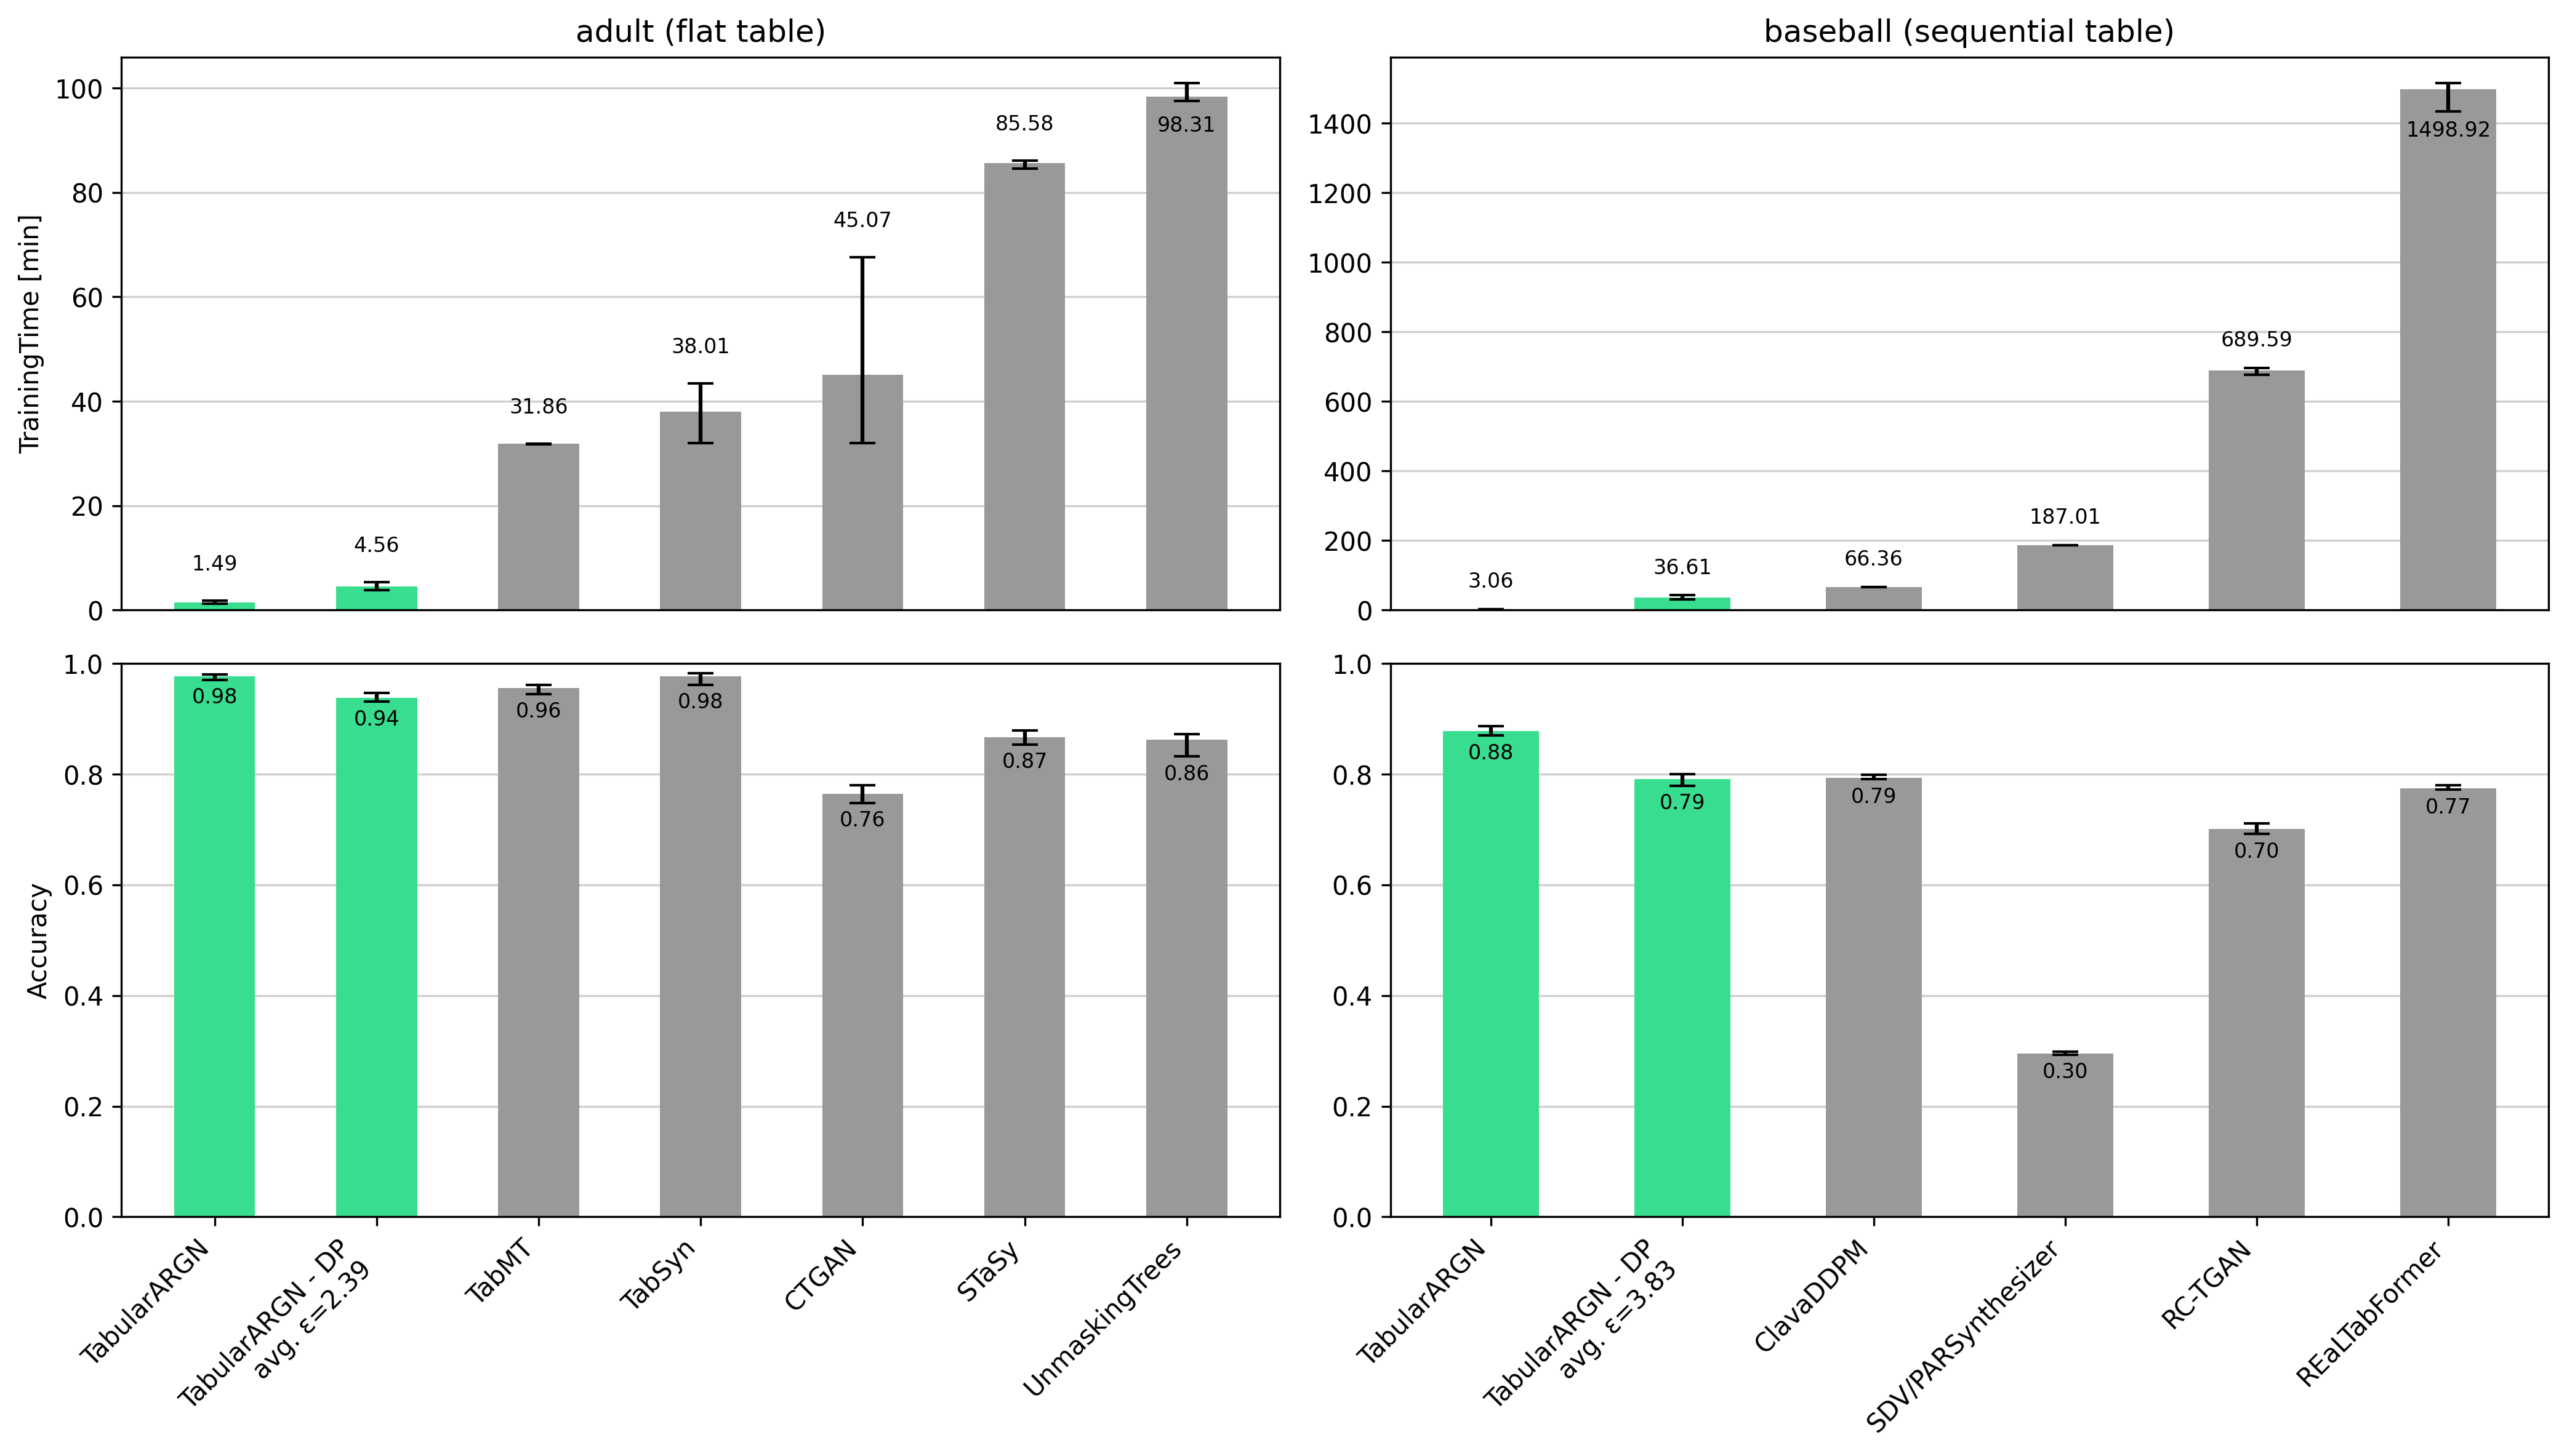
\includegraphics[width=.9\textwidth]{figures/results_mainbody.png}
\caption{플랫 \emph{Adult}(왼쪽) 및 순차 \emph{Baseball}(오른쪽) 데이터 세트에 대한 훈련 시간(상단) 및 정확도(하단). 값은 3회 이상의 실행에 대한 평균입니다. 오류 막대는 최소/최대를 나타냅니다. DP 훈련 유무에 관계없이 TabularARGN이 표시됩니다.}
\label{fig:results}
\end{figure*}

\begin{figure}[t]
\centering
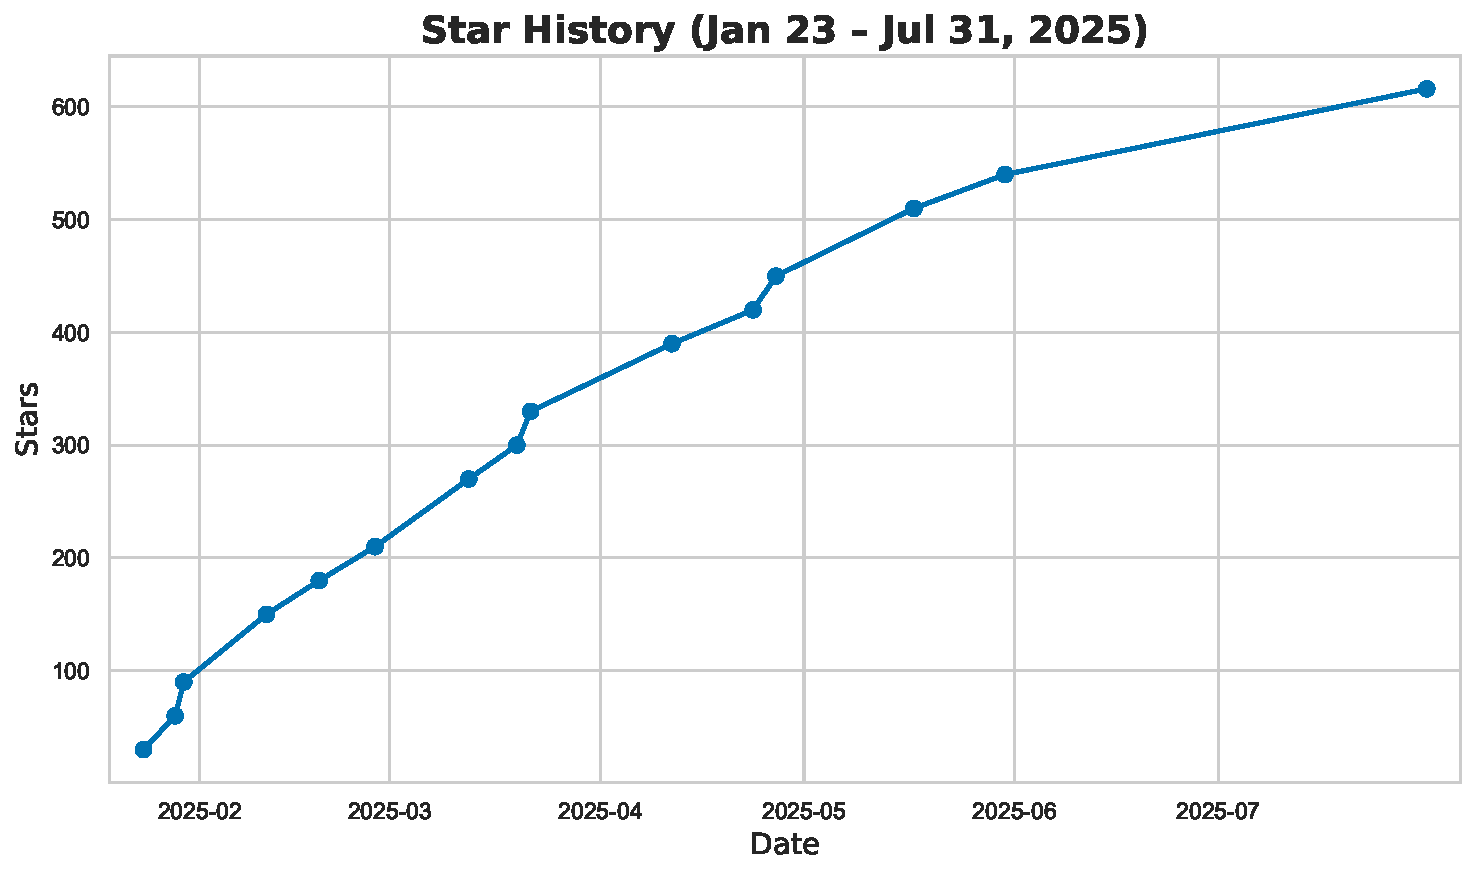
\includegraphics[width=\columnwidth]{figures/star_history.pdf}
\caption{GitHub는 2025년 1월 23일까지 등장합니다. 이후 2025년 7월 31일까지 SDK의 역사를 기록합니다.}
\label{fig:sdk-star-history}
\end{figure}

\begin{figure}[t]
\centering
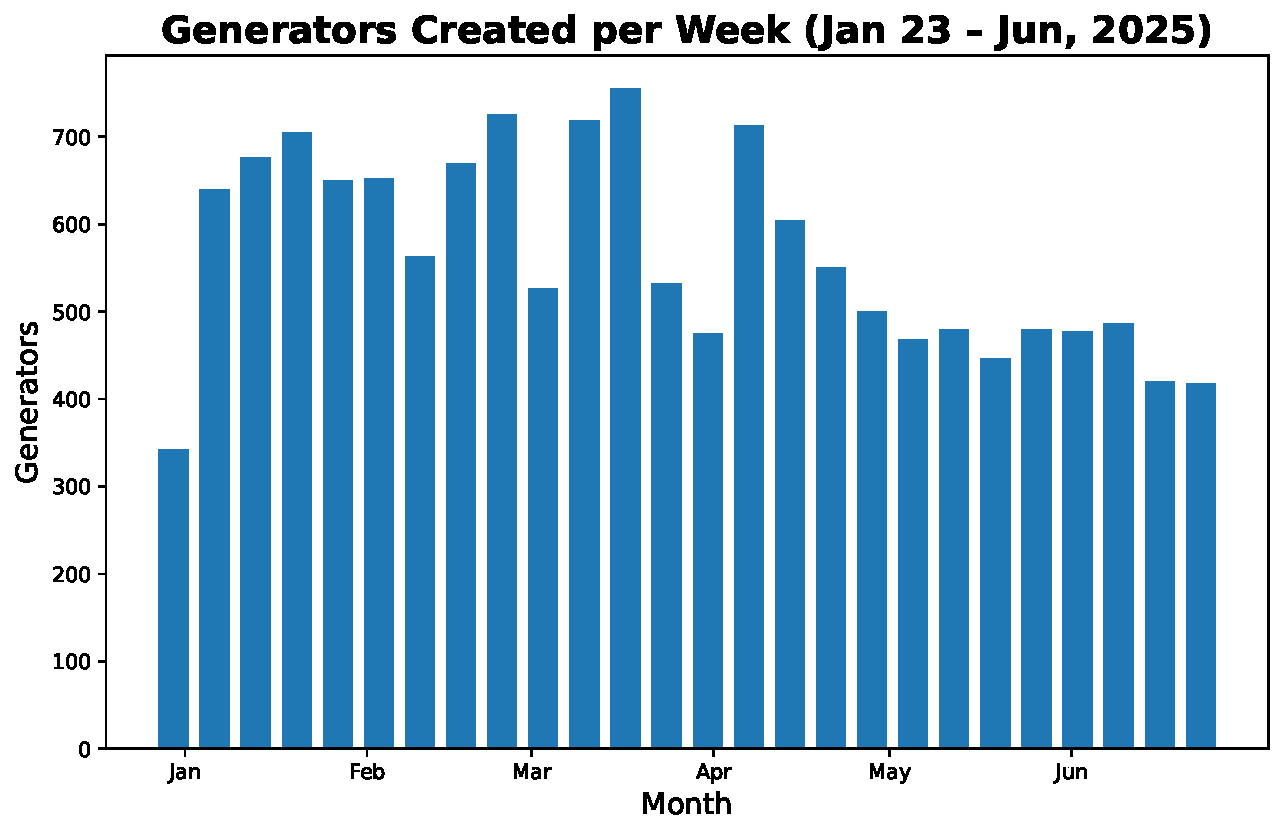
\includegraphics[width=.9\columnwidth]{figures/generators_by_week.pdf}% Reduce the figure size so that it is slightly narrower than the column. Don't use precise values for figure width.This setup will avoid overfull boxes.
\caption{등장일부터 6월까지 MOSTLY AI 조직 외부 사용자가 생성한 주당 생성기 수입니다.}
\label{fig:nb_generators}
\end{figure}


% We spoke about the data bottleneck, how is our SDK addressing that? Opening paragraph.
SDK는 개인정보를 보호하는 합성, 왜곡된 데이터세트의 재조정, 누락된 값의 대치, 공정한 합성 데이터 등 다양한 데이터 문제에 대한 실용적인 솔루션을 제공합니다.
SDK의 실제 영향을 종합적으로 평가하기 위해 우리 작업의 두 가지 보완적인 측면을 자세히 설명합니다.
한편으로는 \cite{tabularargn}가 제시한 실증적 증거가 요약되어 SDK의 핵심 모델인 TabularARGN의 생성 정확성, 강력한 개인 정보 보호 보장 및 효율적인 런타임 측면에서 강력한 성능을 강조합니다.
한편, 2025년 1월 SDK 공개 출시 이후 관찰된 커뮤니티 채택 증가에 대해 논의하여 실용성, 유용성 및 관련성을 입증합니다.

\subsection{합성 데이터 품질}

% There is a rich and growing body of literature on synthetic tabular data generation, with many works focusing on specific data types or modeling challenges. While numerous papers target flat tables \citep{uri16,ank15,qia23}, and others focus on sequential data generation \citep{yoo19-TimeGAN, lin20-DoppelGANger, des21-TimeVAE, zhi24-sdformer, yua24-diffusionts, suh24-timeautodiff}, holistic frameworks that natively support multiple data structures and privacy-preserving features within a unified solution remain rare. The SDK presented in this paper addresses this gap, building on the TabularARGN model introduced by \cite{tabularargn}.


우리 접근 방식의 효율성을 입증하기 위해 이전에 \cite{tabularargn}에서 보고된 주요 경험적 결과를 요약합니다. 여기서 TabularARGN은 평면 및 순차 테이블 형식 데이터 세트 모두에 대한 최첨단 방법에 대해 벤치마킹되었습니다.
평가는 일변량 및 이변량 정확도와 같은 저차 한계 통계를 통해 측정된 통계적 충실도와 DCR(Distance to Closest Record) 공유와 같은 측정항목을 통해 정량화된 개인정보 보호 품질 측면에서 합성 데이터의 품질을 평가하는 \cite{pla21-qa}가 제안한 프로토콜에 따라 수행되었습니다.
이 평가 프로토콜은 \cite{mostlyai-qa}에서 사용할 수 있는 오픈 소스 패키지~\cite{qareport}에서 구현됩니다.
SDK는 이 패키지를 활용하여 앞서 섹션 2에서 설명한 포괄적인 품질 보증 보고서를 생성합니다.

플랫 테이블의 경우 모델을 CTGAN \cite{xu19}, STaSy \cite{kim23-StaSy}, TabSyn \cite{zha24-TabSyn}, TabMT \cite{gul23-TabMT} 및 Unmasking Trees \cite{mcc24-UnmaskingTrees}와 같은 방법과 비교했습니다. 순차 데이터의 경우 벤치마크에는 REalTabFormer \cite{sol23-Realtabformer}, RC-TGAN \cite{gue23-rctgan} 및 ClavaDDPM \cite{pan24-clavaddpm}가 포함되었습니다.
여러 데이터세트를 조사했지만 이 섹션에서는 종단적 플레이어 성능 통계로 구성된 \emph{성인} 인구 조사 데이터세트와 \emph{야구} 데이터세트의 각 데이터 체계에 대해 하나의 데이터세트 결과만 제시합니다.
Figure~\ref{fig:results}는 DP를 사용하여 교육할 때에도 벤치마크에 비해 상당한 속도 향상을 제공하면서 최첨단 성능을 달성하는 TabularARGN의 능력을 강조하는 주요 결과를 보여줍니다. 이는 정확도와 런타임에 부정적인 영향을 미칠 수 있습니다.


\subsection{확장성 및 응용 프로그램 처리}
해당 분야의 상당한 발전에도 불구하고 딥 러닝 기반 표 형식 데이터 생성기의 대부분은 유연성, 확장성 또는 실제 데이터베이스 토폴로지에 대한 지원을 희생하면서 개인 정보 보호 또는 충실도와 같은 문제의 하위 집합만 해결하는 데 여전히 초점을 맞추고 있습니다. 대표적인 예가 DataCebo에서 개발하여 널리 사용되는 비즈니스 소스 Python 라이브러리인 SDV(Synthetic Data Vault) ~\cite{pat16-sdv}입니다. 이 라이브러리는 GAN 및 VAE를 포함한 다양한 생성 모델링 기술을 활용하여 단일 테이블, 다중 테이블 및 시계열 데이터 합성을 위한 도구를 제공합니다. 그러나 벤치마킹 및 실험 평가 \footnote{SDV vs. SDK: \url{https://mostly.ai/blog/a-comparison-of-synthetic-data-vault-and-mostly-ai-part-1-single-table-scenario}의 단일 테이블 시나리오}에서는 SDV가 특정 단일 테이블 사용 사례에서 탁월하지만 더 크거나 복잡한 데이터 세트에서는 확장성 및 성능 제한에 직면할 수 있으며 수동 구성 또는 광범위한 매개 변수 조정이 필요할 수 있음을 보여줍니다.
이 분석을 복잡한 관계형 및 시간적 종속성이 있는 2개의 테이블 데이터 세트로 확장하면 SDV가 이러한 패턴을 캡처하는 데 어려움을 겪는 반면 SDK는 이러한 패턴을 보다 효과적으로 처리하여 이러한 조건 \footnote{SDV vs. SDK: Sequential Scenario at \url{https://mostly.ai/blog/a-comparison-of-synthetic-data-vault-and-mostly-ai-part-2-sequential-scenario}}에서 더 높은 충실도와 유용성을 달성한다는 사실을 관찰했습니다.

% There is currently a vast corpus of literature on tabular data generation, with numerous works individually addressing particular aspects of the problem.
% A large body of papers specifically target vector-structured dataset ("flat" tables) \citep{uri16,ank15,qia23}, while others specialize on sequential data \citep{yoo19-TimeGAN, lin20-DoppelGANger, des21-TimeVAE, zhi24-sdformer, yua24-diffusionts, suh24-timeautodiff}.
% However, to the best of our knowledge, holistic approaches integrating multiple data structures and privacy-preserving features into a unified framework are scarce.
% Our SDK aims at filling this gap by building upon the TabularARGN model introduced by \cite{tabularargn}.

% To illustrate the effectiveness of our SDK in terms of synthetic data quality we summarize key empirical results reported by \cite{tabularargn}.
% In this prior work the authors evaluated TabularARGN across standard benchmarks for both data regimes, flat and sequential, over well-established publicly available datasets, assessing generation accuracy and privacy guarantees \cite{qareport}, as well as runtime performance.
% For flat tables, TabularARGN was evaluated against several state-of-the-art models that leverage different generative approaches, namely, CTGAN \cite{xu19}, STaSy \cite{kim23-StaSy}, TabSyn \cite{zha24-TabSyn}, TabMT \cite{gul23-TabMT}, and Unmasking Trees \cite{mcc24-UnmaskingTrees}.
% For sequential tables, comparisons included REalTabFormer \cite{sol23-Realtabformer}, RC-TGAN \cite{gue23-rctgan}, and ClavaDDPM \cite{pan24-clavaddpm}.
% Although several datasets were examined, in this Section we only present results on one dataset for each data regime, the \emph{adult} census dataset and the \emph{baseball} dataset, comprising longitudinal player-performance statistics.
% More details about the baselines and datasets can be found in Appendix~\ref{app:related_work} and \ref{app:datasets}.
% In Figure~\ref{fig:results} we present the main results, which underscore TabularARGN's ability to achieve state-of-the-art performance while providing significant speed-ups over the benchmarks, even when training with DP, which can negatively impact accuracy and runtime.
% These are crucial requirements in real-world scenarios where computational resources might be limited and high-quality synthetic data must be generated at scale.
% We refer the reader to Appendix~\ref{app:more_results} for detailed experimental setups and full results.

% \begin{figure*} 
%      \centering
%      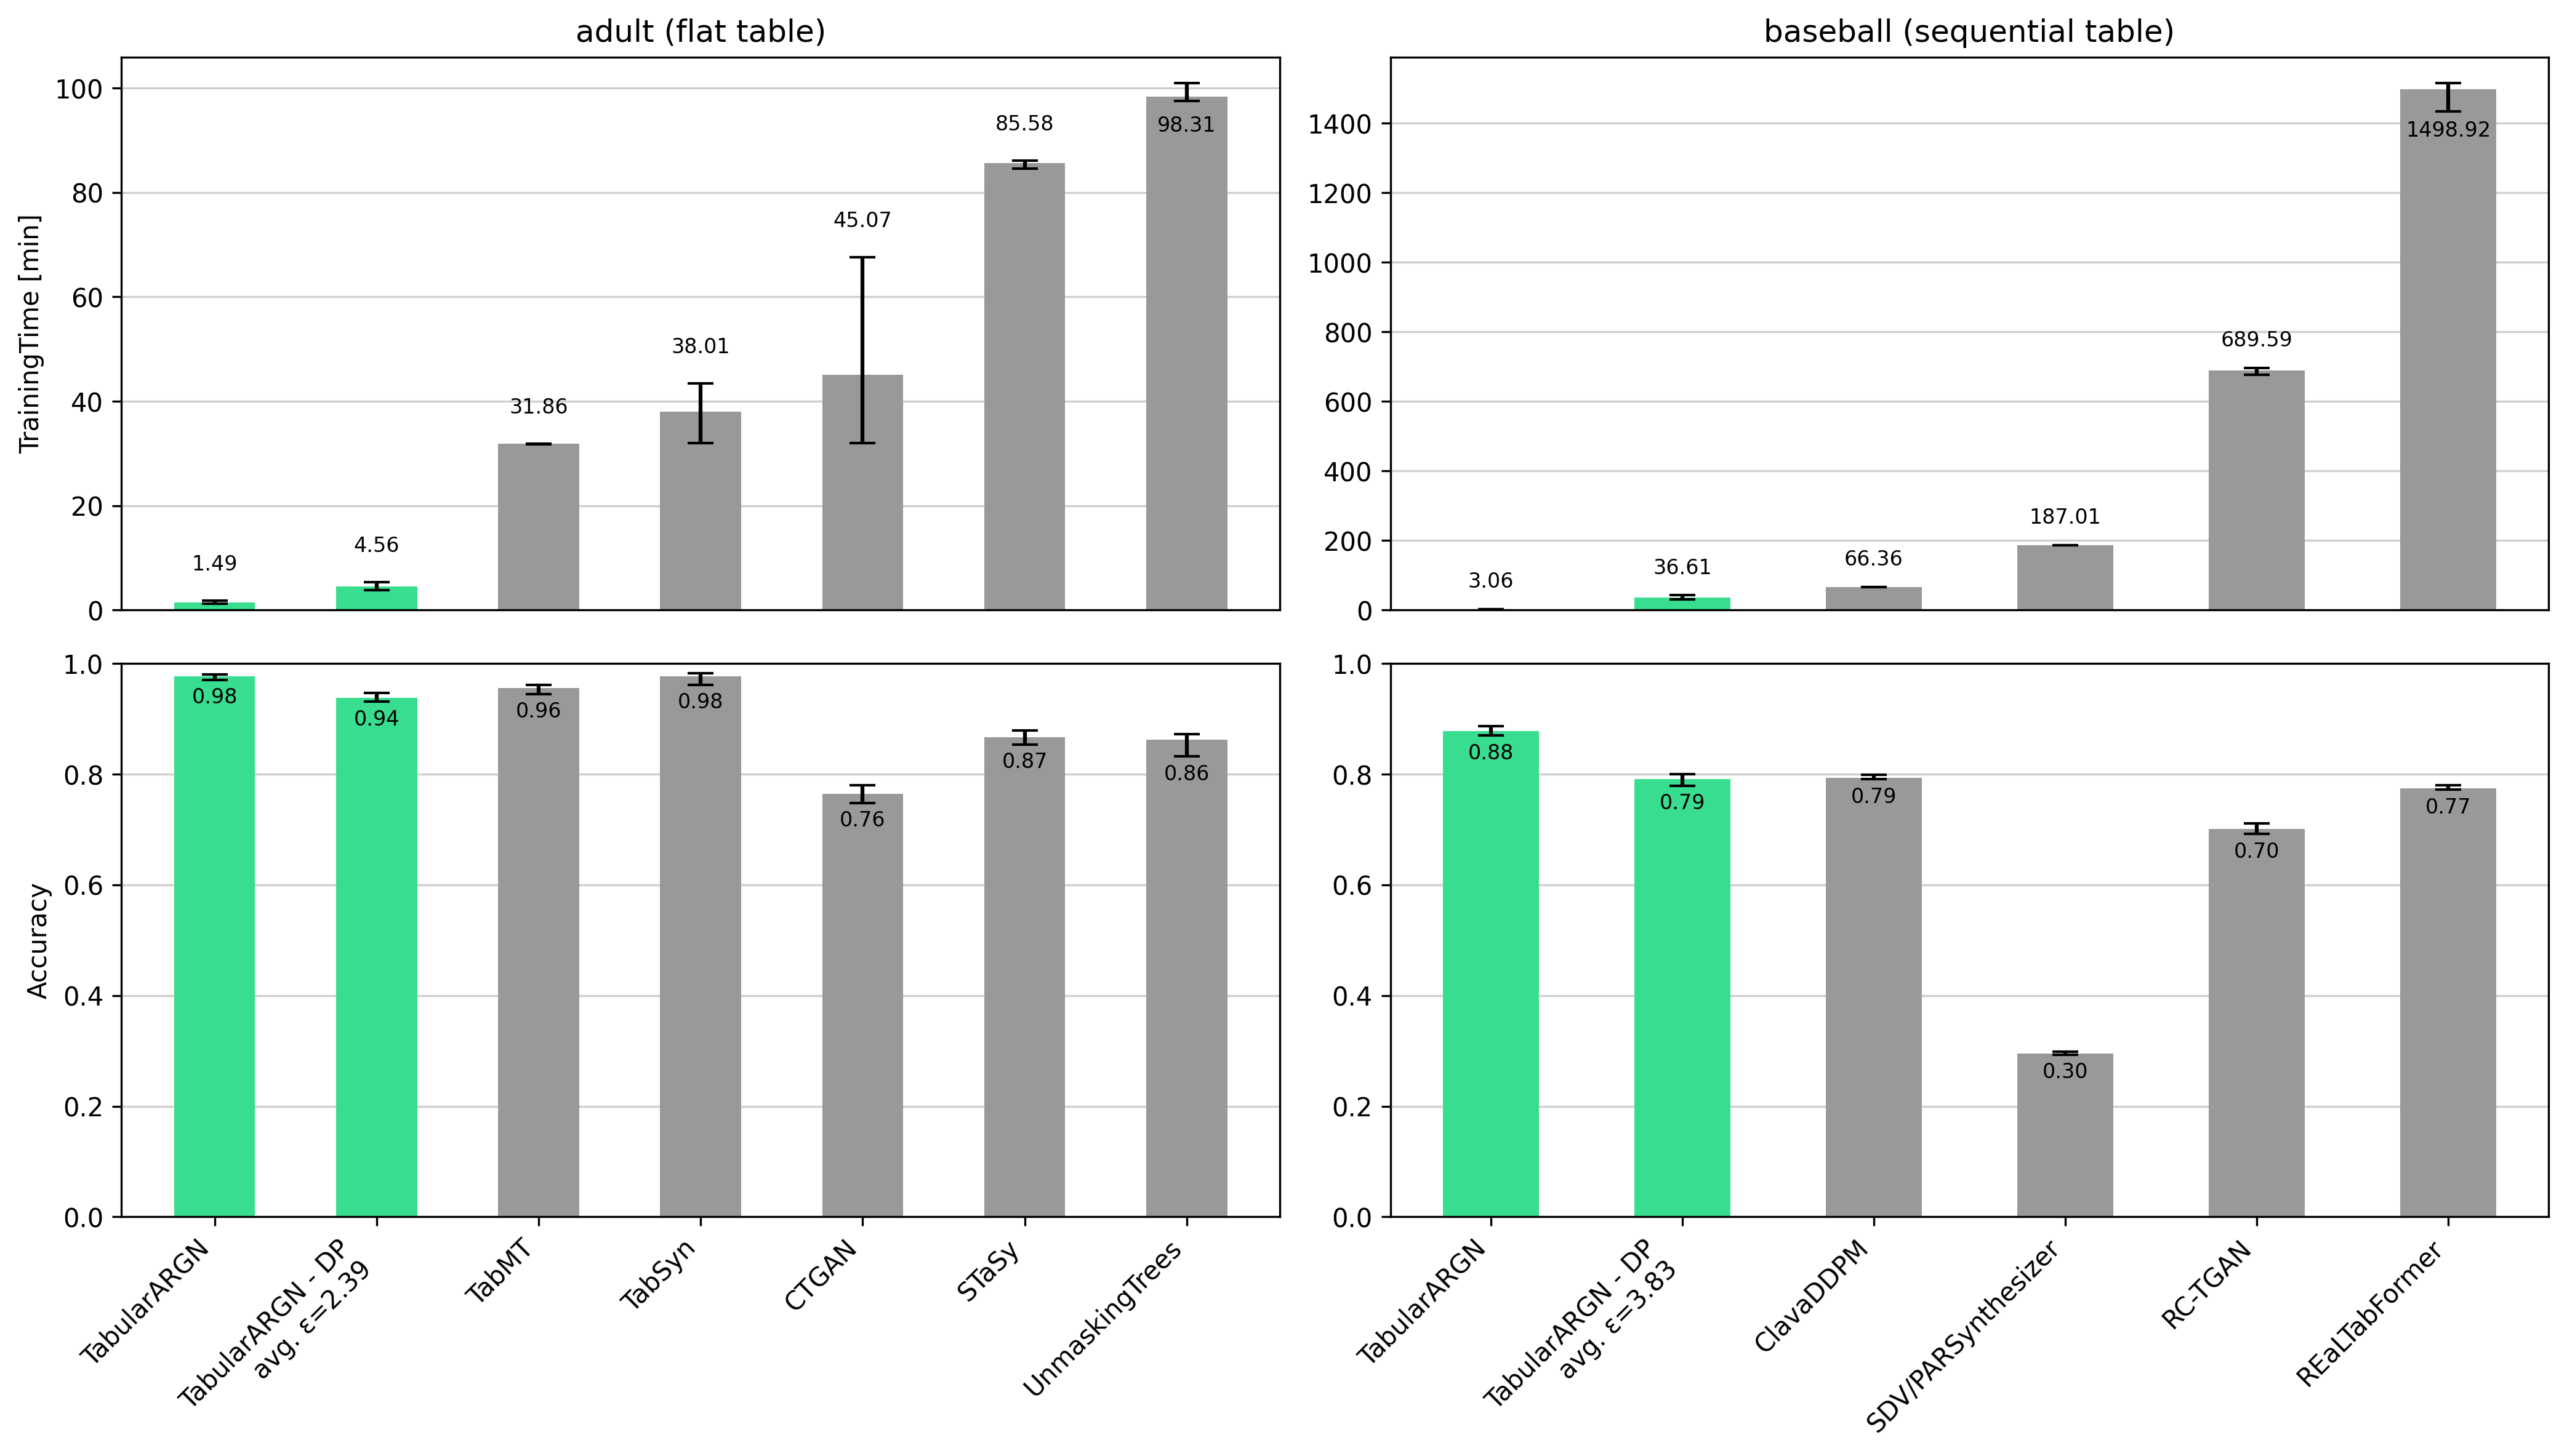
\includegraphics[width=\textwidth]{figures/results_mainbody.png}
%      \caption{Training time (top) and accuracy (bottom) for the flat \emph{Adult} (left) and sequential \emph{Baseball} (right) datasets. Values are averaged over three or more runs; error bars indicate min/max. TabularARGN is shown both with and without DP training.}
%      \label{fig:results}
%      % Let's avoid vskip
% \end{figure*}

\subsection{커뮤니티 채택}

SDK는 2025년 1월 23일 출시된 이후 GitHub에서의 참여가 증가하면서 빠르게 채택되었습니다. Figure~\ref{fig:sdk-star-history}는 출시일부터 7월 31일까지 GitHub 스타의 증가를 추적하며 이는 강력한 관심 지표입니다.
또한 Figure~\ref{fig:nb_generators}에는 MOSTLY AI 조직에 속하지 않은 사용자가 생성한 주당 생성기 수가 표시됩니다.
중요한 것은 이 수치는 클라우드 서비스에서 생성된 생성기만 나타내므로 로컬에서 생성된 생성기를 포함하는 실제 사용량의 하한으로 사용된다는 것입니다.
이는 툴킷에 대한 커뮤니티의 실질적인 참여를 강조합니다.

이미 실제 적용을 추진하는 열정이 커지고 있습니다.
최근 사례로는 기업과 기관이 데이터 서비스 및 분석을 제공하여 데이터에서 실행 가능한 지식을 추출할 수 있도록 하는 것을 목표로 하는 유럽 조직인 Moderate Project에서 개발한 에너지 성능 인증서용 시각화 도구가 있습니다.\footnote{Moderate의 기본 웹사이트: \url{https://moderate-project.eu/in-a-nutshell/}}.
Moderate 팀은 SDK를 지오 클러스터링 도구에 통합하여 이탈리아 피에몬테 지역의 에너지 성능 인증서를 분석하기 위한 시각화 도구를 개발할 수 있었습니다.
기본 데이터는 공개적으로 사용할 수 없으므로 합성 데이터를 활용하여 이 도구를 공개적으로 사용할 수 있도록 합니다.\footnote{시각화 도구는 \url{https://tools.eeb.eurac.edu/epc_clustering/piemonte/}에서 사용할 수 있습니다.}

\paragraph{추가 리소스}
SDK의 모든 주요 기능을 다루는 사용 지침과 광범위한 튜토리얼도 제공되어 모든 수준의 사용자가 SDK를 빠르게 시작하고 전체 기능 \footnote{\url{https://mostly-ai.github.io/mostlyai/tutorials/}}을 탐색할 수 있도록 돕습니다.
